\begin{center}
\begin{longtable}{ |l|l| } 
 \hline
 Attribute & Description\\ 
 \hline
 timestamp & when the event occured\\ 
 \hline
 eventId & ID of the event\\ 
 \hline
 teamId & ID of the team\\ 
 \hline
 teamLevel & level that team has stared or completed\\ 
 \hline
 eventType & type of the event (start or end)\\ 
 \hline
\caption{level-events.csv}
\end{longtable}
\end{center}

Level events appears not to have any missing values.
\begin{figure}[H]
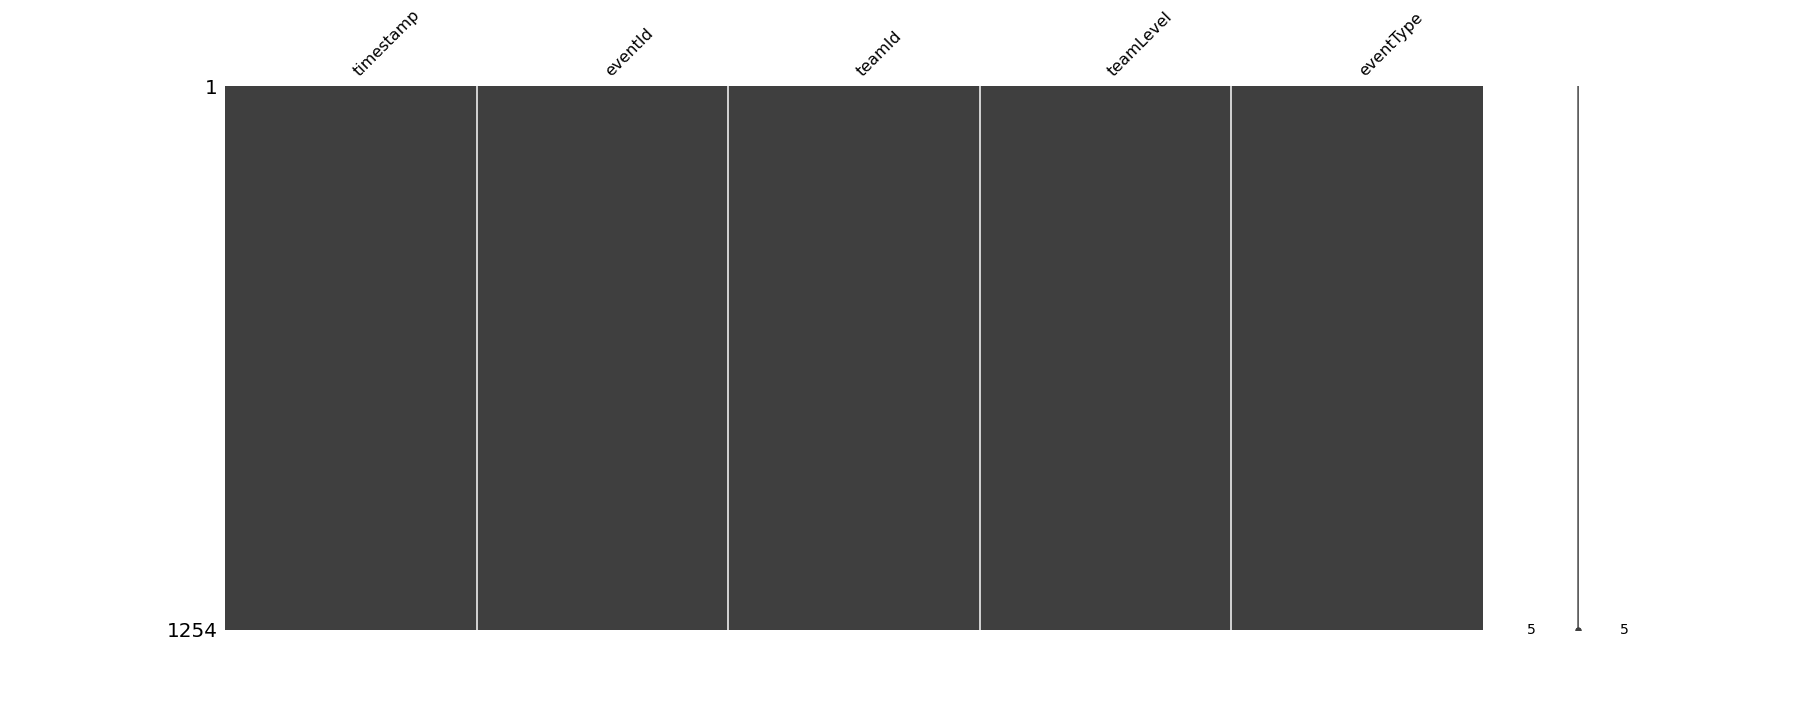
\includegraphics[scale=0.25]{img/Graphs/levelEvents/missingno_levelEvents.png}
\centering
\caption{missingno\_levelEvents}
\label{fig:missingno_levelEvents}
\end{figure}

The time series for level events is unusual. There appears to be 7 spikes, which could indicate when players went up the levels and then it finishing. Other possibility is game events occurring every so often. The graph itself does look different, but the ending seems to be the same as with other graphs. Analysing the graph left to right, we can see how it goes up and down. But at the end, it goes down from the spike, when we would expect it to go back up, it went down again. This seems to confirm that something odd has happened with time series so far.
\begin{figure}[H]
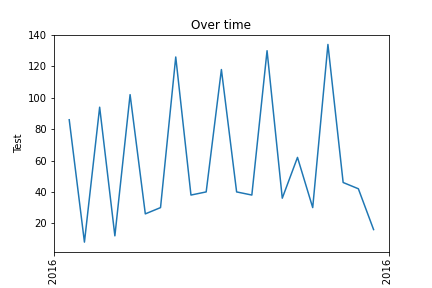
\includegraphics[scale=0.85]{img/Graphs/levelEvents/timeseries_levelEvents.png}
\centering
\caption{timeseries\_levelEvents}
\label{fig:timeseries_levelEvents}
\end{figure}